%%%%%%%%%%%%%%%%%%%%%%%%%
% Imports and Setup     %
%%%%%%%%%%%%%%%%%%%%%%%%%

\input{../lib/hw-setup/tex/HWSetup}
\input{../lib/hw-setup/tex/EngBindings}
\usepackage{cleveref}

\fancyhead[C]{}
\fancyhead[R]{\hyperlink{tableofcontents}{\hmwkClass\ (\hmwkClassInstructor,\ \hmwkClassTime): \hmwkTitle}}
\fancyheadwidth[L]{0.5\headwidth}
\fancyheadwidth[C]{0.0\headwidth}
\fancyheadwidth[R]{0.5\headwidth}

%%%%%%%%%%%%%%%%%%%%%%%%%
% Homework Details      %
% - Title               %
% - Subtitle            %
% - Due Date            %
% - Due Time            %
% - Course              %
% - Section Time        %
% - Instructor          %
% - Author              %
% - Submission Time     %
%%%%%%%%%%%%%%%%%%%%%%%%%

\hwkTitle{Lab05}
\hwkSubTitle{Ludwieg-Tube Experiments on a Free-Flying Cone}
\hwkDueDate{2026-04-17}
\hwkDueTime{23:59:00}
\hwkClass{ENAE464 - 0202}
\hwkClassTime{14:00:00}
\hwkInstructor{Dr. Silbaugh}
\hwkAuthor{Mikołaj Kostrzewa \& Vai Srivastava}
\hwkCompletionDate{
    Experiment Performed: \DTMdate{2026-04-10}\\
    Report Submitted: \DTMtoday
}

\addbibresource{./references.bib}

\begin{document}

\hypertarget{titlepage}{\maketitle}
\thispagestyle{empty}

\pagebreak

%%%%%%%%%%%%%%%%%%%%%%%%%
% Letter of Transmittal %
%%%%%%%%%%%%%%%%%%%%%%%%%

\thispagestyle{empty}

\DTMtoday

\vspace{5.0ex}

Enclosed is the technical report for the \textit{Ludwieg-Tube Experiments on a Free-Flying Cone} laboratory experiment. This report presents the experimental methodology, results, and analysis of flow characteristics and effects for a free-flying cone in a Mach-4 Ludwieg tube.

Please feel free to contact us with any questions regarding the contents of this report.

\vspace{5.0ex}

Respectfully,

Mikołaj Kostrzewa \& Vai Srivastava

%%%%%%%%%%%%%%%%%%%%%%%%%
% Table of Contents     %
%%%%%%%%%%%%%%%%%%%%%%%%%

\pagebreak

\thispagestyle{empty}
\hypertarget{tableofcontents}{\tableofcontents}

\renewcommand{\listfigurename}{Figures}
\listoffigures

\renewcommand{\listtablename}{Tables}
\listoftables

\renewcommand{\listlistingname}{Listings}
\listoflistings

\newpage
\pagenumbering{arabic}

%%%%%%%%%%%%%%%%%%%%%%%%%
% Report                %
%%%%%%%%%%%%%%%%%%%%%%%%%

\section{Abstract} \label{sec:abstract}

% FIXME: write abstract
\lipsum[1]

\section{Introduction} \label{sec:introduction}

The Ludwieg tube is a type of impulse wind tunnel capable of generating high-speed supersonic and hypersonic flows efficiently and cost-effectively, albeit with limited test duration \cite{slaurence2026ludwieg}. Unlike continuous-flow facilities that require large compressors and extensive power infrastructure, the Ludwieg tube operates on a simple principle: a long charge tube is pressurized to the desired fill conditions, then a fast-acting valve or burst diaphragm is opened, allowing an unsteady expansion wave to propagate upstream while accelerating the gas through a converging-diverging nozzle into the test section. This transient operation provides clean, uniform flow conditions ideal for fundamental aerodynamic studies, though the steady test time is typically limited to tens of milliseconds.

When a body travels through a supersonic or hypersonic flow, the fluid cannot be compressed isentropically ahead of the body due to information traveling only at the local sound speed. Instead, discontinuous shock waves form to rapidly compress the flow and redirect it around the obstacle \cite{danderson2023fundamentals}. For slender axisymmetric bodies such as cones, an attached oblique shock wave emanates from the apex, creating a conical shock surface. A remarkable property of supersonic conical flow is that all flow properties along any ray drawn from the cone vertex remain constant, though they vary from ray to ray as the flow is further compressed between the shock and the body surface \cite{slaurence2026ludwieg}. This flow structure is fundamentally different from two-dimensional wedge flows and requires solving the Taylor-Maccoll ordinary differential equation for exact solutions.

Free-flying models offer significant advantages over traditional sting-mounted configurations in wind tunnel testing. Sting supports can introduce flow interference effects that contaminate force measurements, particularly for drag-sensitive geometries or base pressure studies. By eliminating physical support structures, free-flying experiments provide cleaner aerodynamic measurements. However, this approach introduces its own challenges: the model's motion must be tracked with high precision using non-intrusive optical methods, and the short test duration of impulse facilities limits the time available for meaningful acceleration measurements. Recent advances in high-speed digital imaging and automated image processing have made free-flight techniques increasingly practical for quantitative aerodynamic force determination.

\subsection{Theoretical Background} \label{sec:introduction/theory}

\subsubsection{Ludwieg Tube Flow Analysis}

The flow development in a Ludwieg tube involves a complex interaction between unsteady expansion waves and steady isentropic nozzle flow. When the fast-acting valve opens, an expansion wave propagates upstream into the quiescent charge tube at approximately the local sound speed. This expansion accelerates the gas to a subsonic Mach number $M_t$ determined by the area ratio between the charge tube and nozzle throat according to the area-Mach number relationship:

\begin{equation}
    \left(\frac{A_t}{A^*}\right)^2 = \frac{1}{M_t^2} \left[\frac{2}{\gamma + 1}\left(1 + \frac{\gamma - 1}{2}M_t^2\right)\right]^{(\gamma+1)/(\gamma-1)}
    \label{eq:area-mach-tube}
\end{equation}

\noindent where $A_t$ is the charge tube cross-sectional area, $A^*$ is the nozzle throat area, and $\gamma$ is the specific heat ratio. For this equation, the subsonic solution for $M_t$ must be selected.

The pressure and temperature behind the expansion wave, $p_t$ and $T_t$, are related to the original fill conditions by:

\begin{align}
    \frac{p_t}{p_{\text{fill}}} &= \left(1 + \frac{\gamma - 1}{2}M_t^2\right)^{-2\gamma/(\gamma-1)} \label{eq:expansion-pressure} \\
    \frac{T_t}{T_{\text{fill}}} &= \left(1 + \frac{\gamma - 1}{2}M_t^2\right)^{-2} \label{eq:expansion-temperature}
\end{align}

These post-expansion conditions serve as the effective reservoir conditions for the subsequent isentropic expansion through the nozzle. The stagnation pressure and temperature are then:

\begin{align}
    \frac{p_0}{p_t} &= \left(1 + \frac{\gamma - 1}{2}M_t^2\right)^{\gamma/(\gamma-1)} \label{eq:stagnation-pressure} \\
    \frac{T_0}{T_t} &= 1 + \frac{\gamma - 1}{2}M_t^2 \label{eq:stagnation-temperature}
\end{align}

Finally, the freestream static conditions in the test section are determined from the calibrated exit Mach number $M_\infty$ using the isentropic relations:

\begin{align}
    \frac{p_0}{p_\infty} &= \left(1 + \frac{\gamma - 1}{2}M_\infty^2\right)^{\gamma/(\gamma-1)} \label{eq:freestream-pressure} \\
    \frac{T_0}{T_\infty} &= 1 + \frac{\gamma - 1}{2}M_\infty^2 \label{eq:freestream-temperature}
\end{align}

The freestream density and velocity then follow from the ideal gas law and definition of Mach number: $\rho_\infty = p_\infty/(RT_\infty)$ and $V_\infty = M_\infty\sqrt{\gamma R T_\infty}$.

\subsubsection{Supersonic Conical Flow Theory}

The exact solution for supersonic flow over a cone requires solving the Taylor-Maccoll equation, a nonlinear ordinary differential equation with no closed-form analytical solution. Numerical integration is therefore required to obtain the flowfield properties and surface pressure distribution. However, Rasmussen developed accurate analytical approximations that avoid this computational complexity while maintaining excellent agreement with full numerical solutions for slender cones at high Mach numbers \cite{slaurence2026ludwieg}.

For the shock angle $\beta$ (measured from the freestream direction), Rasmussen's approximation is:

\begin{equation}
    \frac{\sin\beta}{\sin\theta_c} \approx \sqrt{\frac{\gamma + 1}{2} + \frac{1}{M_\infty^2\oldsin^2\theta_c}}
    \label{eq:rasmussen-shock}
\end{equation}

\noindent where $\theta_c$ is the cone half-angle. For the pressure coefficient on the cone surface, the approximation is:

\begin{equation}
    \frac{C_p}{\theta_c^2} \approx 1 + \frac{(\gamma + 1)M_\infty^2}{\theta_c^2 + 2} + \frac{(\gamma - 1)M_\infty^2}{\theta_c^2 + 2}\oldln!\left(\frac{\gamma + 1}{2} + \frac{1}{M_\infty^2\theta_c^2}\right)
    \label{eq:rasmussen-cp}
\end{equation}

An important property of slender conical flows is that the pressure coefficient $C_p$ is approximately uniform over the entire cone surface. Consequently, for inviscid flow, $C_p$ is equal to the inviscid drag coefficient $C_{D,\text{inviscid}}$.

\subsubsection{Drag Force Determination}

For a free-flying body subject only to aerodynamic drag, Newton's second law gives $D = ma_x$, where $D$ is the drag force, $m$ is the body mass, and $a_x$ is the acceleration in the flow direction. If the cone's position is tracked over time using high-speed imaging, a quadratic polynomial can be fitted to the position data:

\begin{equation}
    x(t) = a_0 + a_1 t + a_2 t^2
    \label{eq:quadratic-fit}
\end{equation}

The constant acceleration is then simply $a_x = 2a_2$. The drag coefficient is defined as:

\begin{equation}
    C_D \equiv \frac{2D}{\rho_\infty V_\infty^2 A}
    \label{eq:drag-coefficient}
\end{equation}

\noindent where $A$ is the reference area (cone base area, $A = \pi r^2$). Comparison between the experimentally-determined $C_D$ and the inviscid theoretical prediction from Rasmussen's $C_p$ approximation allows estimation of the viscous drag component, which arises from skin friction and boundary layer displacement effects.

\subsection{Experiment Objectives} \label{sec:introduction/objectives}

The specific objectives of this experiment are:
\begin{enumerate}
    \item Determine the freestream flow conditions (Mach number, pressure, temperature, density, and velocity) in the Ludwieg tube test section from the measured fill conditions using isentropic flow relations and expansion wave theory.

    \item Track the position of a free-flying cone over time using high-speed shadowgraph imaging at \qty{10}{kHz} frame rate and automated edge detection algorithms.

    \item Calculate the experimental drag coefficient from the measured cone acceleration by fitting a quadratic polynomial to the position-time trajectory and applying Newton's second law.

    \item Compute the theoretical inviscid drag coefficient using Rasmussen's pressure coefficient approximation for supersonic conical flow.

    \item Visualize the predicted shock wave geometry and compare the theoretical shock angle with the cone geometry observed in experimental images.

    \item Estimate the viscous drag component (skin friction and boundary layer effects) by comparing the experimental drag coefficient with the inviscid theoretical prediction.
\end{enumerate}

\section{Methodology} \label{sec:methodology}

\subsection{Experimental Apparatus} \label{sec:methodology/apparatus}

The experiment was conducted in the University of Maryland Mach-4 Ludwieg tube, an unheated impulse wind tunnel facility. The apparatus consists of a long charge tube connected to a converging-diverging nozzle through a fast-acting valve, as shown in \ref{fig:methodology/apparatus/ludweig-tube}. The charge tube has a cross-sectional area-to-throat area ratio of $A_t/A^* = 11.4$. The nozzle exit Mach number has been calibrated through previous experiments to be $M_\infty = 4.07$, accounting for the effective area reduction due to boundary layer growth on the nozzle walls.

\begin{figure}[H]
    \centering
    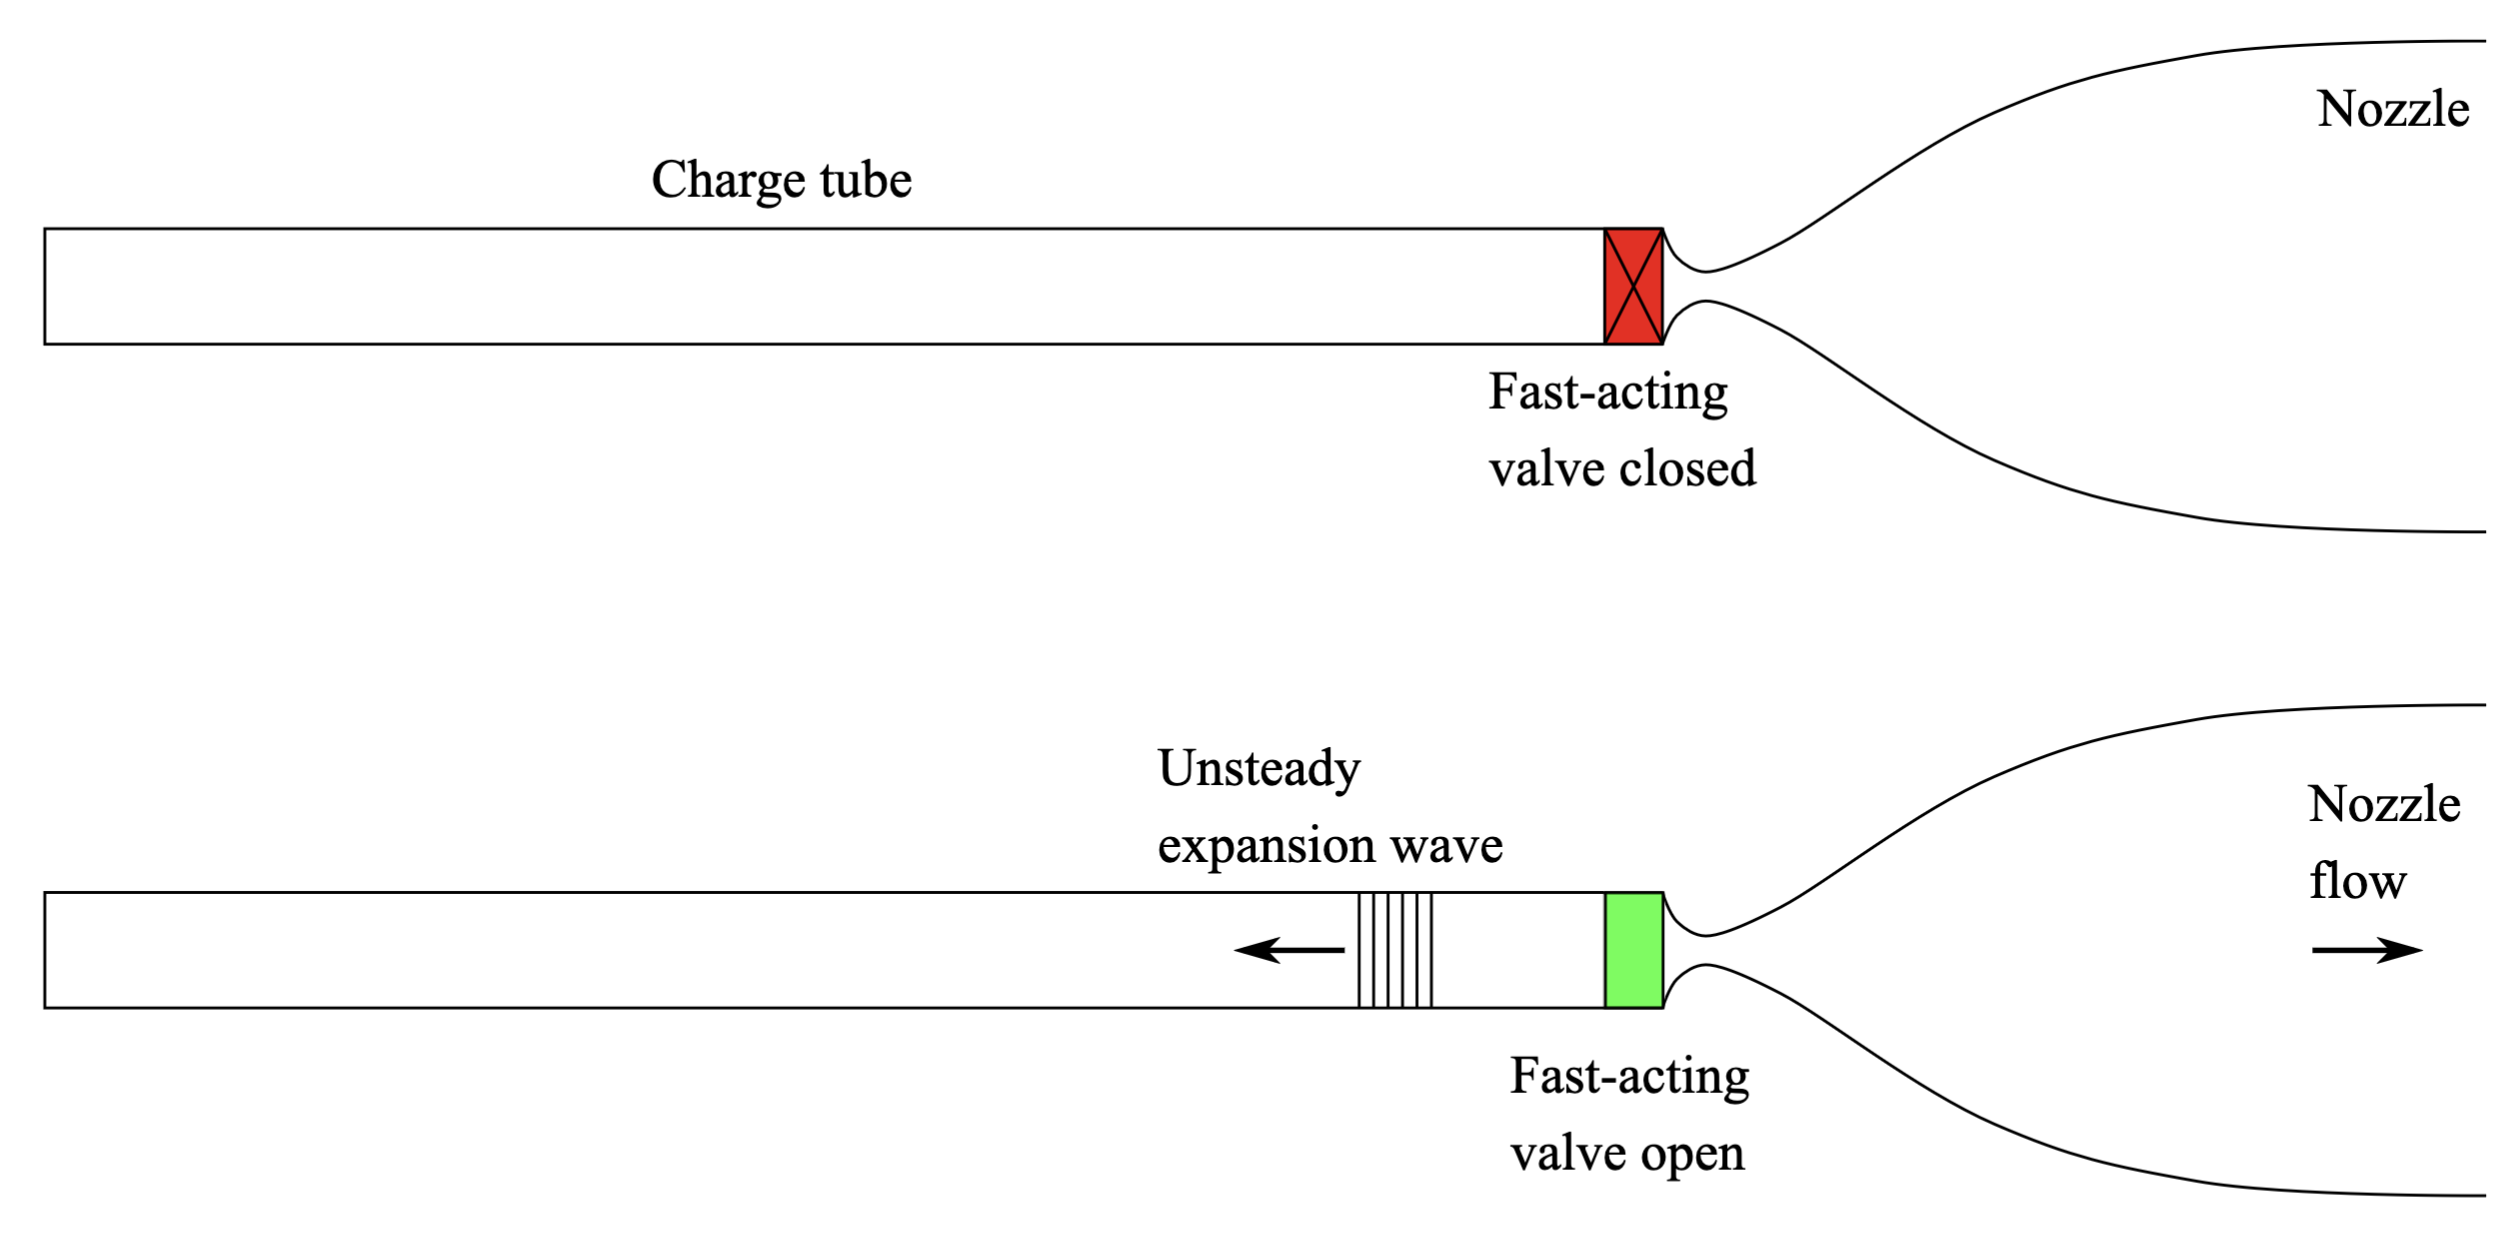
\includegraphics[width=0.65\linewidth]{../assets/ludweig-tube.png}
    \caption{Schematic Diagram of a Ludwieg Tube \cite{slaurence2026ludwieg}.}
    \label{fig:methodology/apparatus/ludweig-tube}
\end{figure}

The test article was a slender cone fabricated from lightweight material with a mass of \qty{1.8}{g}. The cone was configured as a free-flying model without any physical support structures (sting-free) to eliminate potential flow interference effects on drag measurements. The cone half-angle $\theta_c$ and base radius $r$ were determined from the edge detection analysis of experimental images, as detailed in \ref{sec:results/drag/experimental}. High-speed shadowgraph imaging was employed to visualize the cone and surrounding flowfield, with images captured at a frame rate of \qty{10}{kHz} (\qty{0.1}{ms} temporal resolution). The imaging system was calibrated to provide a spatial resolution of \qty{12.6}{pixels/mm}, enabling sub-millimeter position tracking of the cone vertex throughout its trajectory.

\subsection{Operating Procedure} \label{sec:methodology/procedure}

The experimental procedure was as follows:
\begin{enumerate}
    \item The charge tube was filled with air to a pressure of $p_{\text{fill}} = \qty{0.7}{bar}$ (\qty{70}{kPa}) at ambient temperature $T_{\text{fill}} = \qty{296}{K}$.

    \item The cone was positioned in the test section on a release mechanism that would deploy it into the freestream upon flow establishment.

    \item The high-speed shadowgraph imaging system was configured for \qty{10}{kHz} frame rate, providing \qty{0.1}{ms} time resolution between successive images.

    \item The fast-acting valve was opened, initiating an unsteady expansion wave that propagated upstream through the charge tube while accelerating the flow through the converging-diverging nozzle.

    \item Once steady flow conditions were established in the test section (approximately \qtyrange{5}{10}{ms} after valve opening), the cone was released and began its free-flight trajectory.

    \item A total of \num{193} frames were captured during the steady flow period, documenting the cone's position and orientation as it accelerated downstream under the influence of aerodynamic drag.

    \item The experimental images were post-processed using an automated Python-based edge detection algorithm (ported from the original MATLAB implementation) to extract the upper and lower cone edge coordinates in each frame.

    \item Cone vertex positions were determined by fitting linear regressions to the detected edges and computing their intersection point, enabling sub-pixel position accuracy for drag force determination.
\end{enumerate}

\section{Results} \label{sec:results}

\subsection{Freestream Flow Conditions} \label{sec:results/freestream}

The freestream flow conditions in the test section were determined from the measured fill conditions using the equations presented in \ref{sec:introduction/theory}. The experimental parameters were:

\begin{itemize}
    \item Fill pressure: $p_{\text{fill}} = \qty{0.7}{bar} = \qty{70000}{Pa}$
    \item Fill temperature: $T_{\text{fill}} = \qty{296}{K}$
    \item Charge tube area ratio: $A_t/A^* = 11.4$
    \item Calibrated exit Mach number: $M_\infty = 4.07$
    \item Specific heat ratio (air): $\gamma = 1.4$
    \item Gas constant (air): $R = \qty{287}{J/(kg.K)}$
\end{itemize}

\subsubsection{Step 1: Charge Tube Mach Number}

Solving \ref{eq:area-mach-tube} numerically for the subsonic solution yields the Mach number in the charge tube behind the expansion wave:

\begin{equation}
    M_t = \textcolor{red}{[TBD \text{ from Python analysis}]}
\end{equation}

\subsubsection{Step 2: Post-Expansion Conditions}

Using \ref{eq:expansion-pressure,eq:expansion-temperature}, the pressure and temperature behind the expansion wave are:

\begin{align}
    p_t &= p_{\text{fill}} \left(1 + \frac{\gamma - 1}{2}M_t^2\right)^{-2\gamma/(\gamma-1)} = \textcolor{red}{[TBD]} \text{ Pa} \\
    T_t &= T_{\text{fill}} \left(1 + \frac{\gamma - 1}{2}M_t^2\right)^{-2} = \textcolor{red}{[TBD]} \text{ K}
\end{align}

\subsubsection{Step 3: Stagnation Conditions}

Applying \ref{eq:stagnation-pressure,eq:stagnation-temperature}, the stagnation conditions are:

\begin{align}
    p_0 &= p_t \left(1 + \frac{\gamma - 1}{2}M_t^2\right)^{\gamma/(\gamma-1)} = \textcolor{red}{[TBD]} \text{ Pa} \\
    T_0 &= T_t \left(1 + \frac{\gamma - 1}{2}M_t^2\right) = \textcolor{red}{[TBD]} \text{ K}
\end{align}

\subsubsection{Step 4: Freestream Static Conditions}

Finally, using the calibrated exit Mach number $M_\infty = 4.07$ and \ref{eq:freestream-pressure,eq:freestream-temperature}, the freestream static conditions are:

\begin{align}
    p_\infty &= \frac{p_0}{\left(1 + \frac{\gamma - 1}{2}M_\infty^2\right)^{\gamma/(\gamma-1)}} = \textcolor{red}{[TBD]} \text{ Pa} \\
    T_\infty &= \frac{T_0}{1 + \frac{\gamma - 1}{2}M_\infty^2} = \textcolor{red}{[TBD]} \text{ K} \\
    \rho_\infty &= \frac{p_\infty}{RT_\infty} = \textcolor{red}{[TBD]} \text{ kg/m}^3 \\
    a_\infty &= \sqrt{\gamma R T_\infty} = \textcolor{red}{[TBD]} \text{ m/s} \\
    V_\infty &= M_\infty a_\infty = \textcolor{red}{[TBD]} \text{ m/s}
\end{align}

These calculated freestream conditions provide the reference state for all subsequent drag coefficient and Reynolds number calculations.  The complete results are summarized in \ref{tab:results/freestream/summary}.

\begin{table}[H]
    \centering
    \caption{Calculated freestream flow conditions. Values in red will be filled from Python analysis output.}
    \label{tab:results/freestream/summary}
    \begin{tabular}{lcc}
        \toprule
        \textbf{Parameter} & \textbf{Value} & \textbf{Units} \\
        \midrule
        $M_t$ & \textcolor{red}{[TBD]} & --- \\
        $p_t$ & \textcolor{red}{[TBD]} & Pa \\
        $T_t$ & \textcolor{red}{[TBD]} & K \\
        $p_0$ & \textcolor{red}{[TBD]} & Pa \\
        $T_0$ & \textcolor{red}{[TBD]} & K \\
        $M_\infty$ & 4.07 & --- \\
        $p_\infty$ & \textcolor{red}{[TBD]} & Pa \\
        $T_\infty$ & \textcolor{red}{[TBD]} & K \\
        $\rho_\infty$ & \textcolor{red}{[TBD]} & kg/m\textsuperscript{3} \\
        $a_\infty$ & \textcolor{red}{[TBD]} & m/s \\
        $V_\infty$ & \textcolor{red}{[TBD]} & m/s \\
        \bottomrule
    \end{tabular}
\end{table}

\subsection{Drag} \label{sec:results/drag}

\subsubsection{Theoretical} \label{sec:results/drag/theoretical}

The theoretical inviscid drag coefficient was calculated using Rasmussen's pressure coefficient approximation (\ref{eq:rasmussen-cp}). The required cone geometry parameters---half-angle $\theta_c$ and base radius $r$---were extracted from the edge detection analysis of the experimental images, as described in \ref{sec:results/drag/experimental}.

\paragraph{Cone Geometry}

From the median values across all \num{193} frames:

\begin{align}
    \theta_c &= \textcolor{red}{[TBD]} \text{ rad} = \textcolor{red}{[TBD]}^\circ \\
    r &= \textcolor{red}{[TBD]} \text{ mm} = \textcolor{red}{[TBD]} \text{ m} \\
    A &= \pi r^2 = \textcolor{red}{[TBD]} \text{ m}^2
\end{align}

\paragraph{Rasmussen Pressure Coefficient}

Applying \ref{eq:rasmussen-cp} with $M_\infty = 4.07$ and the measured cone half-angle:

\begin{equation}
    C_p = \theta_c^2 \left[1 + \frac{(\gamma + 1)M_\infty^2}{\theta_c^2 + 2} + \frac{(\gamma - 1)M_\infty^2}{\theta_c^2 + 2}\oldln!\left(\frac{\gamma + 1}{2} + \frac{1}{M_\infty^2\theta_c^2}\right)\right] = \textcolor{red}{[TBD]}
\end{equation}

For slender conical flows, the surface pressure coefficient is uniform and equals the inviscid drag coefficient:

\begin{equation}
    C_{D,\text{inviscid}} = C_p = \textcolor{red}{[TBD]}
\end{equation}

\paragraph{Theoretical Drag Force and Acceleration}

Using the calculated freestream dynamic pressure $q_\infty = \frac{1}{2}\rho_\infty V_\infty^2$ and cone base area:

\begin{align}
    D_{\text{inviscid}} &= C_{D,\text{inviscid}} \cdot q_\infty \cdot A = \textcolor{red}{[TBD]} \text{ N} \\
    a_{\text{inviscid}} &= \frac{D_{\text{inviscid}}}{m} = \frac{\textcolor{red}{[TBD]}}{\qty{0.0018}{kg}} = \textcolor{red}{[TBD]} \text{ m/s}^2
\end{align}

This theoretical prediction assumes inviscid flow and provides a baseline for comparison with the experimental drag measurement.

\subsubsection{Experimental} \label{sec:results/drag/experimental}

% FIXME: determination of drag coefficient and actual drag force on the cone
\lipsum[1]

\subsection{Shock Angle} \label{sec:results/shock-angle}

The theoretical shock angle was calculated using Rasmussen's approximation (\ref{eq:rasmussen-shock}) for the measured cone half-angle and freestream Mach number. Applying this relationship:

\begin{equation}
    \sin\beta = \sin\theta_c \sqrt{\frac{\gamma + 1}{2} + \frac{1}{M_\infty^2\oldsin^2\theta_c}}
\end{equation}

With $M_\infty = 4.07$, $\theta_c = \textcolor{red}{[TBD]}$ rad, and $\gamma = 1.4$, the shock angle is:

\begin{equation}
    \beta = \textcolor{red}{[TBD]} \text{ rad} = \textcolor{red}{[TBD]}^\circ
\end{equation}

The shock wave forms a conical surface emanating from the cone vertex. In a two-dimensional side view (as captured in the shadowgraph images), this conical shock appears as two straight rays at angle $\beta$ measured from the freestream direction. The theoretical shock geometry is visualized in \ref{fig:results/shock-angle/theoretical-shock}, where the predicted shock rays (red dashed lines) are overlaid on the detected cone edges (blue solid lines) from a representative experimental frame.

The shock angle $\beta$ is consistently larger than the cone surface angle $\theta_c$, as required for attached shock conditions. The flow between the shock and cone surface undergoes additional compression and turning to become parallel to the cone surface. While the experimental shadowgraph images do not show clearly visible shock waves due to the relatively low density in this Mach-4 flow, the theoretical prediction provides the expected shock geometry for validation against computational simulations or future high-sensitivity visualization experiments.

\begin{figure}[H]
    \centering
    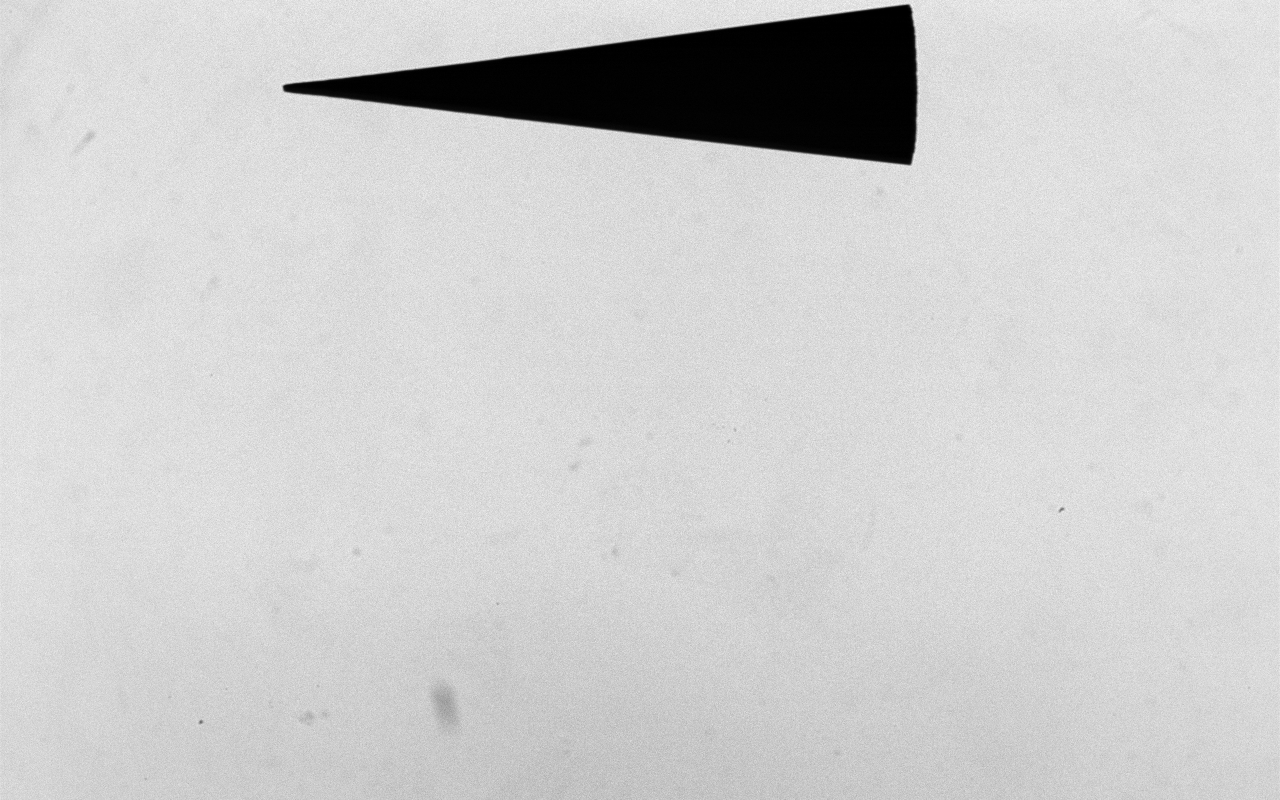
\includegraphics[width=0.75\linewidth]{../outputs/figures/theoretical-shock.png}
    \caption{Theoretical shock shape overlaid on cone edges from experimental imaging. The blue solid lines show the detected cone edges, the green circle marks the calculated vertex position, and the red dashed lines represent the theoretical shock rays at angle $\beta = \textcolor{red}{[TBD]}^\circ$ from the freestream direction.}
    \label{fig:results/shock-angle/theoretical-shock}
\end{figure}

\section{Analysis and Discussion} \label{sec:analysis}

\subsection{Comparison Between Theoretical and Experimental Drag Effects} \label{sec:analysis/comparison}

% FIXME: comparison of derived drag values with Cp and theoretical CD
\lipsum[1]

\subsection{Viscous Component of Drag} \label{sec:analysis/viscous}

% FIXME: estimation of viscous drag component on the cone (based on experimental drag coefficient and Cp)
\lipsum[1]

\section{Summary and Conclusions} \label{sec:summary}

% FIXME: summarize and conclude
\lipsum[1]

\section{References} \label{sec:references}

\printbibliography[heading=none]

\section{Appendices} \label{sec:appendices}

\subsection{Data} \label{sec:appendices/data}

For the sake of brevity, the raw measurement data will not be displayed in this report. However, in the spirit of completeness, the repository containing the complete data, source code, and notes for this report can be found at \href{https://www.github.com/vaisriv/enae464-lab05}{github:vaisriv/enae464-lab05}.

\subsection{Code} \label{sec:appendices/code}

Similarly, only the code files that are key to the analysis are included below, and can be accessed in full in the aforementioned \href{https://www.github.com/vaisriv/enae464-lab05}{GitHub repository}.

\begin{codeblock}
    \centering
    \caption{Data Analysis Script.}
    \mintinline{bash}{./src/index.py}
    \inputminted{python}{../src/index.py}
    \label{lst:appendices/code/index}
\end{codeblock}

% render all references
\nocite{*}

\end{document}
